\section{Evénements}\label{sec:evenements}
\subsection{Composition et exécution de programme}

Un programme est composé de trois parties principales :
\begin{itemize}
    \item \textbf{Code machine} : Instructions représentant la logique des traitements.
    \item \textbf{Espace de données} : Contient les données manipulées par le programme (variables globales, tableaux, variables dynamiques obtenues via \texttt{malloc}).
    \item \textbf{Stack} : Héberge les données de travail courantes (variables locales) et les informations d'appels de fonctions imbriquées.
\end{itemize}

Ces composantes sont liées par des adresses, utilisées pour les branchements, appels et retours de fonction, accès aux cases d'un tableau, et manipulations de la stack. Pour s'exécuter, elles doivent être placées en mémoire principale.

Le processeur suit un cycle \textit{fetch-decode-execute} :
\begin{itemize}
    \item \textbf{Fetch} : Récupération de l'instruction courante depuis la mémoire.
    \item \textbf{Decode} : Décodage de l'instruction pour déterminer le traitement.
    \item \textbf{Execute} : Exécution de l'instruction, mise à jour des registres et/ou de la mémoire.
\end{itemize}

L'\textit{instruction pointer} (ou \textit{program counter}) contient l'adresse de l'instruction courante et est mis à jour après chaque instruction (soit par incrémentation, soit par branchement). L'état du programme à un moment donné est déterminé par :
\begin{itemize}
    \item Les valeurs des registres
    \item Le contenu de la stack
    \item Le contenu de l'espace de données
    \item L'\textit{instruction pointer}
\end{itemize}

Une sauvegarde de ces éléments représente un instantané de l'état du programme, permettant de reprendre l'exécution là où elle s'est arrêtée.

\begin{figure}[h]
    \centering
    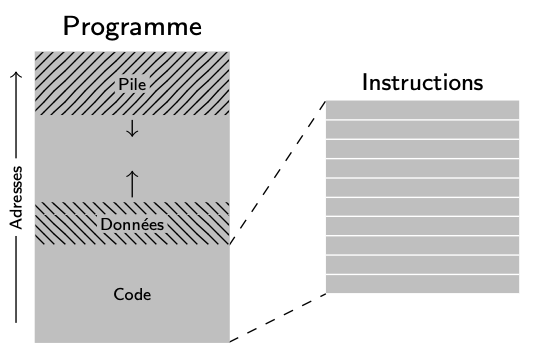
\includegraphics[width=0.4\textwidth]{Images/View/program-view.png}
    \caption{Program view}
\end{figure}

\subsection{Concept de base – évènement}

Lorsqu’un programme est exécuté par le processeur, deux questions se posent :
\begin{itemize}
    \item \textbf{Erreur d'instruction} : Doit-on redémarrer la machine ou gérer l’anomalie pour limiter les dégâts ?
    \item \textbf{Activité de périphérique externe} (e.g. frappe au clavier) : Peut-on suspendre temporairement le programme en cours pour traiter l’activité ?
\end{itemize}

Ces situations sont résolues par la gestion des \textbf{évènements}, mécanismes permettant au processeur de brancher vers du code spécifique en réponse à un évènement.

\subsection{Exceptions (évènements synchrones)}
Origine interne, résultant de l’exécution de l’instruction courante :
\begin{itemize}
    \item \textbf{Code opératoire invalide} : Opcode non reconnu par le processeur.
    \item \textbf{Division par zéro} : Nécessité d’un dénominateur non-nul.
    \item \textbf{Instruction privilégiée} : Niveau de privilège insuffisant pour exécuter l’instruction.
    \item \textbf{Instruction non-chargée en mémoire} : Le système d’exploitation charge la partie manquante en mémoire.
\end{itemize}

\subsection{Interruptions (évènements asynchrones)}
Origine externe, provoquées par un signal de périphérique :
\begin{itemize}
    \item \textbf{Frappe de clavier} : Fermeture d’un circuit électronique, générant une interruption.
    \item \textbf{Fichier prêt pour lecture} : Le contrôleur de disque génère une interruption après lecture des données.
    \item \textbf{Réception d’un paquet réseau} : La carte réseau génère une interruption après réception complète d’un paquet.
    \item \textbf{Erreur du matériel} : Anomalies détectées (e.g. température excessive).
    \item \textbf{Signal d’horloge} : Interruption générée 32.768 fois par seconde pour suivre le temps.
\end{itemize}


\subsection{Conséquences possibles pour le programme}

Le système d'exploitation doit gérer les évènements survenus pendant l'exécution d'un programme. Selon la nature de l'évènement, deux décisions peuvent être prises :

\begin{itemize}
    \item \textbf{Évènement récupérable} : Après traitement, il est possible de continuer l'exécution du programme.
    \item \textbf{Évènement irrécupérable} : La faute ne peut être corrigée, et il est nécessaire de terminer le programme.
\end{itemize}

\subsubsection{Evènement récupérable}

Lorsqu'un évènement récupérable survient, il est crucial de préserver l'état du processeur. Le gestionnaire d'évènements doit sauvegarder le contexte du programme suspendu (registres et stack) avant de traiter l'évènement. Cette sauvegarde est similaire à celle d'un appel de fonction.

% Le gestionnaire d'évènements sauvegarde uniquement les registres pertinents (e.g. $r_, $s_, $t_). Certaines architectures de processeur utilisent un mécanisme de basculement de stack pour éviter les interférences.

La continuation peut être :
\begin{itemize}
    \item \textbf{Reprise} : Retenter l'exécution de l'instruction qui a causé l'évènement.
    \item \textbf{Poursuite} : Passer à l'instruction suivante.
\end{itemize}

Les interruptions sont généralement des évènements récupérables avec poursuite, car elles n'affectent pas l'instruction en cours. Les exceptions comme les appels systèmes (e.g. \texttt{syscall}, \texttt{int}) sont également des évènements récupérables avec poursuite.

Par exemple, une interruption causée par une frappe au clavier est traitée en lisant le code de la touche depuis un port d'entrée/sortie, le traduisant en caractère, puis le transférant au programme destinataire, souvent la fenêtre active dans une interface graphique.

\subsubsection{Evènement irrécupérable}

Lorsqu'un évènement irrécupérable survient, le programme ne peut plus continuer. Une sauvegarde complète du contexte d'exécution est effectuée pour le débogage.

Le programme acquiert diverses ressources (mémoire, descripteurs de fichiers, sockets) au cours de son exécution. Ces ressources doivent être libérées lorsque le programme est terminé.

Les étapes de gestion d'un évènement irrécupérable incluent :
\begin{itemize}
    \item Affichage d'une notification à l'utilisateur décrivant le problème rencontré.
    \item Sauvegarde du contexte dans un fichier (e.g. \texttt{coredump}) ou envoi par mail à un serveur de rapports de crash.
    \item Libération du processeur, permettant la continuation d'un autre programme via un \textit{context switch}.
\end{itemize}


\subsection{Mécanismes de déroutement}

Chaque architecture de processeur spécifie et implémente son mécanisme de déroutement pour la gestion des évènements. Deux techniques principales sont utilisées :

\begin{itemize}
    \item \textbf{Déroutement avec registre de cause} : Un registre indique la cause de l'évènement, permettant au gestionnaire d'évènements de déterminer l'action appropriée.
    \item \textbf{Vectorisation} : Différents types d'évènements sont associés à des adresses spécifiques dans une table de vecteurs, chaque adresse pointant vers le code de gestion correspondant.
\end{itemize}

La technique utilisée influence l'organisation et les responsabilités du code du gestionnaire d'évènements.


\subsubsection{Registre de cause}

Le registre de cause encode les évènements survenus lors du cycle d’exécution courant, mettant à jour les bits pour les exceptions et interruptions. Si au moins un bit est positionné, le processeur réalise un déroutement vers une adresse précise.

Le gestionnaire d’évènements doit :
\begin{itemize}
    \item Lire le contenu du registre de cause.
    \item Tester et traiter les bits des interruptions en attente (bits à 1).
    \item Traiter les exceptions stipulées par le code d’exception.
\end{itemize}

Cette technique permet au système d’exploitation de déterminer l’ordre de priorité des traitements des différents évènements. La fonction principale du gestionnaire d’évènements doit être placée à l’adresse de déroutement définie par le processeur au démarrage du système.

Pour permettre la continuation du programme, l’adresse de l’indicateur d’instruction courante est sauvegardée dans un registre dédié (e.g. Exception Program Counter en MIPS32).


\subsubsection{Vectorisation}

Dans la vectorisation, chaque type d’évènement est associé à un numéro unique (e.g. interrupt vector), identifiant une entrée dans une table de descripteurs (e.g. interrupt descriptor table). Cette table référence la fonction de traitement spécifique (interrupt handler) à invoquer.

Au terme d’un cycle d’exécution, le processeur :
\begin{itemize}
    \item Consulte les numéros d’évènement survenus.
    \item Invoque, dans un ordre déterminé, les fonctions de gestion correspondantes.
\end{itemize}

Le code de chaque fonction de gestion se concentre uniquement sur l’évènement correspondant, avec l’ordre d’invocation des exceptions géré par le processeur.

Au démarrage, le système d’exploitation initialise la table des descripteurs et la référence au processeur via une instruction privilégiée (e.g. \texttt{lidt} en x86).


